% !TeX program = lualatex
% !TeX root = main.tex

\chapter{Graph distance and generation}
\emph{%
This chapter begins with general use cases of graphs. The graph-based distance metric is then described together, as well as some adaptations. The chapter concludes with a discussion about the creation of a graph based on points in space.
}\label{chap:graph}

\section{Introduction}
Graphs $G = (V, E)$ were introduced in chapter~\ref{chap:topics} as a set of nodes $V$ and a list of edges $E$. Edges can have different directions, so that $(v_i, v_j), (v_j, v_i) \in E$, but $(v_i, v_j) \neq (v_j, v_i)$. The same applies to edge weights $w_{i\,j} \neq w_{j\,i}$. Weights are also denoted as $w_{v_i \, v_j}$. A path $\tau: v_i \leadsto v_j$ is a sequence of edges which connects two nodes $v_i$ and $v_j$ (similar concept as density reachability).

%Königsberger Brücken
The first usage of graphs in analysing a problem is thought to be in the famous paper by Leonhard Euler about the Seven Bridges of Königsberg from 1736. The problem was, if it is possible to cross the river Pregolya using all seven bridges of Königsberg once. He proved the impossibility of this task.

%Einsatzbereiche
Today, graph theory is an indispensable tool for logistical optimisation and planning, for example the (time-\,/\,cost-) optimal way of distributing goods with $m$ transporters to $n$ customers. Calculating the shortest or less time consuming way between two locations in a route guidance system is done with graphs. Popular social networks or network-like services embody a graph-like structure (relationship between people) and can therefore be analysed via graphs. Facebooks Graph Search%
\footnote{\url{https://www.facebook.com/about/graphsearch}}%
 and Open Graph framework%
 \footnote{\url{https://developers.facebook.com/docs/opengraph/overview/}}%
 emphasises this with their names.
But there are many other areas of application for graph theory and graph algorithms.

\vspace{3em}

%Darstellung, Speicher
Typical ways of storing graphs in memory are either
\begin{description}
\item[adjacency lists,] where each node has a list of his adjacent nodes and the corresponding weight, or
\item[adjacency matrices,] where each matrix entry $m_{i\,j}$ stands for an edge from node $i$ to node $j$, its value the corresponding weight of the edge.
\end{description}
%
The data structure choice depends, as always, on memory constraints and algorithm design using the graph. Figure~\ref{fig:graphexamples} shows a visualisation of a simple graph accompanied by its representation as adjacency list and matrix.

\begin{figure}[h]
%\centering
	\begin{subfigure}[b]{0.25\textwidth}
		\centering
		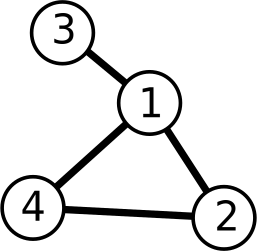
\includegraphics[width=\textwidth]{pix/simple_graph.pdf}
		\caption{Simple graph}
		%\label{fig:gull}
	\end{subfigure}
	\hfill
	\begin{subfigure}[b]{0.25\textwidth}
		\raggedright
		\qquad \begin{description} \itemsep -0.5em
			\item[1:] 2, 3, 4
			\item[2:] 1, 4
			\item[3:] 1
			\item[4:] 1, 2
		\end{description}
		\caption{Adjacency list}
		%\label{fig:gull}
	\end{subfigure}
	\hfill
	\begin{subfigure}[b]{0.25\textwidth}
		\centering
		$\begin{matrix}
			0&1&1&1\\ 1&0&0&1 \\ 1&0&0&0 \\ 1&1&0&0
		\end{matrix}$
		\caption{Adjacency matrix}
		%\label{fig:gull}
	\end{subfigure}
	%\hfill
\caption{Graph representation examples}\label{fig:graphexamples}
\end{figure}

\section{Clustering with graphs}
There are two basic concepts in how to cluster a dataset with the aid of a graph:
\begin{itemize}
\item Direct clustering with the graph structure, and
\item Deriving of features based on the graph, then clustering based on those features.
\end{itemize}
%
The main difference is the sort of clustering algorithm that can be used. Direct clustering requires a graph algorithm whose results are the final clusters. Using feature clustering is indirect, but every possible clustering algorithm can be used, if the derived features (for example a distance) are compatible. A few direct clustering approaches are now presented, to show some possibilities of graph algorithms, to better understand and compare to the feature derivation clustering used in this thesis.

\begin{description}
\item[Single link edge length] One of the simplest ways to directly cluster a graph based on its structure is to use agglomerative hierarchical clustering with single link edge length. This means that in each iteration the nodes connected by the edge with the lowest edge weights are joined in the tree, until all nodes are in one cluster.

\item[Minimum Spanning Trees]
A minimum spanning tree (MST) of a graph is a set of edges with accumulated minimum edge weight, so that every node can reach every other node through a path over those edges. Now whenever an edge is removed, this tree splits in two distinct trees without connection between them, also called connected components. Edge removal can then be iteratively applied until there are enough clusters, or until some other criterion is fulfilled. Selection of the edge to be removed can for example be based on the weight of the edge (remove edge with the highest weight), or a combination of edge length and cluster size like in~\cite{Muller2012}.

%subsection*{Normalized Cut}
\item[Normalized Cut]
Another way are normalized cuts, which seem to be often used in tasks involving image segregation, like in \cite{Shi2000}. The edge weights of an \enquote{image graph} are based on the differences between each pixel. Either every pixel connects to all other pixels in the whole picture, or (more often) every pixel connects to all adjacent pixels. The clustering idea is similar to minimum spanning trees: split the graph in two connected components based on the value of the cut, which equals the sum of the weights of the removed edges. This produces quite good results, but is prone to cut small, isolated groups of nodes in the graph. Thus the value of the normalized cuts is based on the sum of the removed edges versus the sum of the untouched edges. Cuts with minimum value are optimal and lead to more stable partitions.
\end{description}
%
The graph algorithm used for clustering in this paper yields distances between the nodes, which then are used in DBSCAN for clustering.

\section{Distances based on structural and attribute similarities}
The algorithm \emph{SA-cluster} described in the paper \enquote{Graph clustering based on structural\,/\,attribute similarities} by \textcite{Zhou2009} is based on the idea, that nodes close to each other should have many different paths between them. The examples from the previous section only utilise the structure of the graph, but no additional information from the nodes. Very different attributes like timestamps, gender, color, ..., or in this case text, can be further used to determine the closeness of nodes, and thus give better clusters. SA-cluster uses the graph structure and enhances it with the provided attributes to calculate node similarities. The paper also describes a way of automatically adjust the influence of different attributes based on their contribution the the clustering. Because only $text$ is used, there is no need to use it here.

%section~\ref{sec:graph_generation}

%The algorithm operates on a graph whose nodes have attributes: $G = (V, E, \Lambda)$. The only attribute used in this thesis is $text$, but more are possible. 

Figure~\ref{fig:sa} shows a graph with five nodes consisting of two subgraphs with text attributes. The similarity between node 1 and node 4 or node 5 would be $0$, because there is no path between them. But they have the exact same text attribute values, so they should have some similarity. The idea now is to generate additional paths between nodes who have matching attribute values. This is done by creating additional nodes for every possible attribute value, whose edges then connect to nodes having this value. These additional nodes $N_a$ and edges $E_a$ are called \emph{augmented} nodes\,/\,edges, the graph they create $G_a = (N_a, E_a)$ accordingly augmented graph, and the algorithm operates on the unified graph $G \cup G_a$. All following mentions of nodes, edges, and the graph in general are assumed to mean the unified case.
%
\begin{figure}[b]
\centering
	\begin{subfigure}[b]{0.40\textwidth}
		\centering
		\includegraphics[width=\textwidth]{pix/SA1.pdf}
		%\caption{Simple graph}
		%\label{fig:gull}
	\end{subfigure}
	\hfill
	\begin{subfigure}[b]{0.05\textwidth}
	\centering	
	$$\Rightarrow$$\\
	\hspace*{\fill} \\
	\hspace*{\fill}
	\end{subfigure}
	\hfill
	\begin{subfigure}[b]{0.40\textwidth}
		\centering
		\includegraphics[width=\textwidth]{pix/SA2.pdf}
		%\caption{Simple graph}
		%\label{fig:gull}
	\end{subfigure}
	%\hfill
\caption[Transition to the augmented graph.]{Example of nodes with tags, and the corresponding augmented graph.}\label{fig:sa}
\end{figure}
%

The distance between two nodes is now determined by a random walk. A random walk model on a graph starts at a node $v_i$ and then follows $l$ edges at random; $l$ is called the length of the walk. A possibility distribution about how likely other nodes are reached emerges when this is done often enough. By assigning each edge $e_{i\,j}$ a possibility $w_{i\,j} = p_{i\,j}$ describing how likely this edge is used to transition to the next node, the possibility distribution can be calculated by summing up all probabilities of every path with length $l$.

\begin{align}
p(\tau) &= \prod_{e \in \tau} p(e)
\end{align}
%
Summing up all paths between two nodes $v_i$ and $v_j$ with length $l$:
\begin{align}
p(v_i, v_j)=\sum_{\substack{\tau: v_i \leadsto v_j\\lenght(\tau) = l}} p(\tau)
\end{align}
%
is the specific probability of reaching $v_j$ from $v_i$ through paths of length $l$.


%Example:
\begin{figure}%[h]
		\centering
		\includegraphics[width=0.5\textwidth]{pix/transition_ex.pdf}
		\caption[Graph with transition probabilities.]{Example graph with transition probabilities.}
		\label{fig:graph_for_examples}
\end{figure}

As an example this is shown in table~\ref{tbl:RW} for different path lengths based on the example graph in figure~\ref{fig:graph_for_examples}. The distribution diverges after a few iterations, regardless of where the walk was started. In this particular case, the probabilities diverges towards $[0.125, 0.250, 0.250, 0.375]$.

Having probabilities for choosing edges, independent of earlier transition choices makes this a \emph{markov chain}\cite{Aldous2002}. The adjacency matrix can also be called markov matrix, transition matrix or probability matrix $P$, because $w_{i\,j} = p_{i\,j}$. Markov chains as stochastic processes are well understood, thus every probability $p(v_j, v_i, l)$ of reaching $v_j$ from $v_i$ in a random walk with length $l$ can be calculated trough simple matrix multiplications of the transition matrix:

\begin{align}
p(v_j, v_i, l) &= P^l (v_j, v_i)
\end{align}

Table~\ref{tbl:RW2} shows an example of this using the transition matrix instead of finding and listing all possible paths. It can be seen that the distributions are very inconsistent in the first iterations, even on this small graph. The probability distribution which diverges over time is obviously no good indication of a distance between nodes.

Finally the distance between two nodes $f(v_i, v_j)$ based on a random walk model is the sum of each distribution for a finite number of iterations $l$ (which also means the sum of every possible path $\leq l$):

\begin{align}
f(v_i, v_j) &= \sum_{\substack{\tau: v_i \leadsto v_j\\lenght(\tau) \leq l}} p(\tau) \: c \: (1-c)^{lenght(\tau)}
\end{align}
%
or in matrix form
\begin{align}
R^l &= \sum^{l}_{y=1} c \: (1-c)^y \: P^y\\
		&= c \: (1-c)^l \: P^l + R^{l-1}
\end{align}
%
$c \in (0,1)$ is called restart probability and models the case that the random walker just stops. Because $w_{i\,j}$ is not necessary equal to $w_{j\,i}$, the resulting distance may differ $d(v_i, v_j) \overset{?}{=} d(v_j, v_i)$. To keep it simple, every distance is the average of $d(v_j, v_i)$ and $d(v_i, v_j)$ (respectively $R_d = \frac{R+R^T}{2}$). In table~\ref{tbl:RW3} the final distances for the example graph by using the random walk model can be found.

\section{Edge weights}
Assignment of the edge weights is based on the individual number of edges per attribute and node, and attribute weights for each attribute. There is a distinction between nodes and attributed nodes (edges) in calculating the edge weights. Therefore, the normal nodes are called structure nodes ($v_i, v_j$), and the nodes generated from the attributes are called augmented nodes ($v_k^a$). $v_k^a$ describes the node based on the $a^{th}$ value of attribute $k$. Similarly $v_k$ is the set of all nodes based on attribute $k$. There are edges $(v_i, v_k^a), (v_k^a, v_i)$ if and only if $v_i$ has the $a^{th}$ value of attribute $k$ set. Structure edges have an attribute weight of $\omega_0$, while the augmented edges of attributes $k_1, \dots, k_m$ have attribute weights $\omega_1, \dots, \omega_m$.

\subsubsection*{Example}
Node $v_{42}$ has the attribute $text = [red, green]$. This means there are augmented nodes $v_{text}^{red}$ and $v_{text}^{green}$ with edges $(v_{42}, v_{text}^{red}), (v_{42}, v_{text}^{red}) \in E$. There are of course also edges from the augmented nodes to the structure node, but with different weights. See also for example figure~\ref{fig:sa}.
%The number of text edges for $v_{42}$ is written as $|N(v_{text})(v_{42})|$ and would be $2$.

\vspace{1em}
\noindent
The following transition probabilities are the edge weights between nodes as defined by \textcite{Zhou2009}. $|N(v)|$ is the number of outgoing edges of $v$.
%
\begin{align}
\intertext{structure edge $(v_i, v_j)$}
w_{v_i \, v_j} &=
\begin{cases} 
	\frac{\omega_0}{|N(v_i)| \, \cdot \, \omega_0 + \omega_1 + \dots + \omega_m} &\text{if } (v_i,v_j) \in E\\
	0 &otherwise
\end{cases}
\intertext{attribute edge $(v_i, v_k^a)$}
w_{v_i \, v_k^a} &=
\begin{cases} 
	\frac{\omega_k}{|N(v_i)| \, \cdot \, \omega_0 + \omega_1 + \dots + \omega_m} &\text{if } (v_i,v_k^a) \in E\\
	0 &otherwise
\end{cases}
\intertext{attribute edge $(v_k^a, v_{j})$}
w_{v_k^a \, v_{j}} &=
\begin{cases} 
	\frac{1}{|N(v_k^a)|} &\text{if } (v_k^a, v_{j}) \in E\\
	0 &otherwise
\end{cases}
\end{align}
%
There are no edges between attribute nodes.

The edge weights $w_{i\,j}$, thus $P_A$, should represent a probability distribution with the requirements $0 \leq w_{i\,j} \leq 1$ and $\sum_{j} w_{i\,j} = 1$. All edges from attribute nodes obviously fulfil this requirement. But edges from structure nodes have various summed probabilities. This will be exemplary shown after the following proposed edge weights. $N_k(v_i)$ is the number of edges to any attribute node $v_k^a$; similarly $N_0(v_i)$ for edges to structure nodes. 
%
\begin{align}
\intertext{structure edge $(v_i, v_j)$}
w_{v_i \, v_j} &=
\begin{cases} 
	\frac{\omega_0}{\sum_m \omega_m |N_m(v_i)|} &\text{if } (v_i,v_j) \in E\\
	0 &otherwise
\end{cases}
\intertext{attribute edge $(v_i, v_k^a)$}
w_{v_i \, v_k^a} &=
\begin{cases} 
	\frac{\omega_k}{\sum_m \omega_m |N_m(v_i)|} &\text{if } (v_i,v_k^a) \in E\\
	0 &otherwise
\end{cases}
\end{align}
%
Attribute weights now proportionally control the different edge weights.

\subsubsection*{Example}
This example demonstrates the difference between the old edge weights as described in \cite{Zhou2009} and the new proposed edge weights. The basis is a node with 3 structure edges and 6 attribute edges of attribute 1. Attribute weights are $\omega_0 = 0.7, \omega_1 = 0.3$. This results in the following weights per edge respectively the sum of the probabilities:


\begin{center}
\footnotesize
\begin{tabular}{rrrr}
\toprule
 & $w_{structure}$ & $w_{attribute}$ & $\sum_{j} w_{i\,j}$\\
\midrule
old & $0.106$ & $0.045$ & $0.59$\\
new & $0.179$ & $0.077$ & $1.00$\\
\bottomrule
\end{tabular}
\end{center}
%
Attribute edge weights can be any positive number.

\section{Super nodes}
The proposed calculation scheme based on matrix multiplications is easy to adopt, because there are many fast and relatively easy to use libraries dealing with (sparse) matrix multiplication.

Dealing with datasets containing hundreds of thousands, or millions of documents require huge amounts of memory when using matrix multiplications. 
For example a full matrix of 25,000 points with single-precision floating point numbers (32~Bit) , needs approximately 4.6~GB of space. This number grows quadratic with the count of documents. Even with sparse matrices, which store only values other than $0$, the matrices grow very big after a few iterations of multiplications. Too big for the test system in use with 4~GB RAM.

The datasets used have an interesting characteristic: many points with the same attributes are at the same position (or at least less than a few meters apart). It is safe to assume that they end up in the same cluster. All this occurrences of structure nodes with the exactly same attributes within very close proximity are in each case combined to super nodes.

The idea behind super nodes is to reduce the amount of nodes and edges in the graph, thus reducing the space needed, without changing the local characteristics of the edges and their weights to much. Incoming\,/\,outgoing edges involving the same node are being merged. Every incoming edge now represents $k$ normal edges, and has $k$-times the priority of a normal edge. $k$ is based on the number of nodes $N_w$ consolidated by the super node based on the following equation:

\begin{align}
k =  \frac{\sqrt{9 \cdot N_w}}{2}
\end{align}
%
Without this adjustment the super nodes gained too much incoming probability, leading to low distances to super nodes, but to high to other nodes. Edges to and from augmented nodes are handled the same way. Figure~\ref{fig:w_nodes} shows this concept.

Using super nodes helped to reduce the needed amount of memory drastically, so that even one million points can be computed with the test system. Previously this had theoretically required over 7~TB of RAM.

\begin{figure}[h]
\centering
	\begin{subfigure}[b]{0.4\textwidth}
		\centering
		\includegraphics[width=\textwidth]{pix/w_nodes1.pdf}
		%\caption{Simple graph}
		%\label{fig:gull}
	\end{subfigure}
	\hfill
	\begin{subfigure}[b]{0.4\textwidth}
		\centering
		\includegraphics[width=\textwidth]{pix/w_nodes2.pdf}
		%\caption{Simple graph}
		%\label{fig:gull}
	\end{subfigure}
	%\hfill
\caption[Transition from normal nodes to a super node.]{Example of a transition from normal nodes to super nodes. All edges count as 1, except for the ones from and to the newly created super node.}\label{fig:w_nodes}
\end{figure}

\section{Generating the graphs}\label{sec:graph_generation}
The described graph algorithm operates on a structure graph based on the location data and different augmented graphs for every other used attribute (text data in this case). Creating the augmented graphs is easy: 
\begin{enumerate}
\item Create an augmented node for every individual value of every attribute
\item Create edges between structure nodes and augmented nodes
\end{enumerate}
%
That is all to represent the relationship between structure node and augmented node. The relationship between structure nodes should be based upon the closeness of each other and the relative density of the points. This means, there should be no edge between nodes to far away, and there should be a rather high connectivity in areas with many points.

The following two approaches come to mind, where an edge is created to either 
\begin{enumerate}
\item all the $n$-nearest nodes, or 
\item all nodes in an $eps$-neighbourhood.
\end{enumerate}
%
Both reflect the closeness and density aspects, but unfortunately suffer for these exact same reasons. They usually connect highly in dense areas, but very little elsewhere. Connectivity sometimes reached a point where every node in an area was connected to every other node. Which did not work well for the algorithm, was calculation intensive, and reduced the meaning (closeness) of an edge. 

Beside this general problem, approach 1 sometimes forms \enquote{bubbles}: sets of highly interconnected nodes without edges to surrounding nodes, in high density areas. Raising $n$ would prevent this, at the cost of even greater interconnected areas. And approach 2 was very sensitive in choosing $eps$. Nodes inside a neighbourhood were usually very highly interconnected; nodes outside very usually not connected at all.\footnotetext[3]{\url{https://en.wikipedia.org/wiki/File:Delaunay_circumcircles.png}}

\begin{wrapfigure}{r}{0.42\textwidth}
	\centering
	\includegraphics[width=0.38\textwidth]{pix/Delaunay_circumcircles.png}
	\caption[Delaunay triangulation example]{Delaunay triangulation example{\protect\footnotemark}}
	\label{fig:delaunay_example}
\end{wrapfigure}
%
Because of those problems, the final method of creating the structure graph is a \emph{Delaunay triangulation}. A triangulation is a set of non-intersecting edges, whose only shapes are triangles. A Delaunay triangulation is a special triangulation, such that no node is inside the circumcircle of any triangle. A circumcircle is the circle whose center is equidistant to all three points of the triangle. Figure~\ref{fig:delaunay_example} shows an example together with the circumcirles of the triangles. Because of this requirement the minimum angle of all the angles of the triangles is maximised. This results in well distributed looking edges, whose nodes are close to each other, without too much interconnectivity in highly populated areas. 

Areas with low point density will also be well connected. This is a problem, because those points can be rather far away from each other. Deleting edges above a certain threshold lowers this and results are much better, but the bottom line is:

The case of extreme connectivity versus no connectivity, in both approaches \enquote{$n$-nearest nodes} and \enquote{$eps$-neighbourhood}, is now traded to good connectivity versus mild connectivity. Examples of the triangulations, together with colour-coded edge lengths can be seen in the description of the datasets in section~\ref{sec:datasets}.%\todo{more DT}
